\documentclass[12pt,a4paper]{extarticle}
\usepackage[utf8]{inputenc}
\usepackage[T5]{fontenc}
\usepackage{geometry}
\geometry{a4paper, left=1.5cm, right=1cm, top=1.5cm, bottom=1.5cm, headheight=20pt, headsep=15pt, footskip=28pt}
\usepackage{enumitem}
\usepackage{amsmath}
\usepackage{amssymb}
\usepackage{diagbox}
\usepackage[most]{tcolorbox}
\newcommand{\khongxacdinh}{\text{KXĐ}}
\newcommand{\blackbox}[1]{\texorpdfstring{\fcolorbox{black}{black}{\textcolor{white}{#1}}}{#1}}
\usepackage{tikz}
\definecolor{bookblue}{RGB}{58,90,172}
\definecolor{book}{RGB}{58,90,172}
\definecolor{myblue}{RGB}{200,40,40}
\newcommand{\bluecheck}{\textcolor{myblue}{\checkmark}}
\newtcolorbox{formulaBox}{colback=gray!5,colframe=bookblue,boxrule=0.8pt,arc=2mm}
\newtcolorbox{notebox}{colback=blue!3,colframe=myblue,boxrule=0.8pt,arc=2mm}
\usetikzlibrary{patterns, patterns.meta} % Thêm patterns.meta vào đây
% Gọi package nằm trong thư mục con template
\usepackage{../template/mngocbox}

\begin{document}

% Sử dụng ngoặc vuông [...] để thay đổi linh hoạt các thông số
\makeheadbox[headerright={Chương 1},chude={Bài 3},tieude={Các đường tiệm cận},dinhdang={Giải tích},lop={12 },gv={Nguyễn Lê Minh Ngọc}]

\vspace{2em}
\makeheading{I}{Kiến thức cần nhớ}
\subsection*{1. Đường tiệm cận ngang}
\begin{doublelinebox}
    Đường thẳng $y = y_0$ được gọi là đường tiệm cận ngang của đồ thị hàm số $y = f(x)$ nếu:\\
    $\displaystyle\lim_{x \to +\infty} f(x) = y_0$ hoặc $\displaystyle\lim_{x \to -\infty} f(x) = y_0$.
\end{doublelinebox}
\begin{center}
    % Hình 1: Tiệm cận ngang bên phải
    \begin{minipage}{0.48\textwidth}
        \centering
        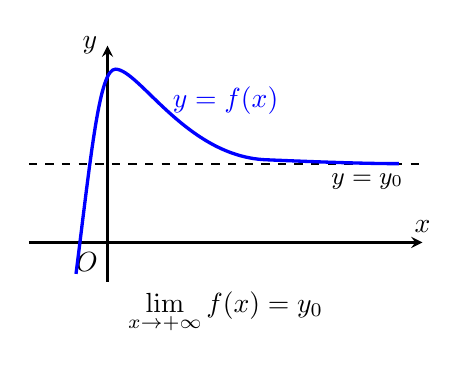
\begin{tikzpicture}[scale=1.0, >=stealth]
            % Axes
            \draw[->, thick] (-0.5,0) -- (4.5,0) node[above] {$x$};
            \draw[->, thick] (0.5,-0.5) -- (0.5,2.5) node[left] {$y$};
            \node[below left] at (0.5,0) {$O$};
            
            % Dashed horizontal line y = y_0
            \draw[dashed, thick] (-0.5,1.0) -- (4.5,1.0);
            \node[below, font=\small] at (3.8,1.0) {$y = y_0$};
            
            % Curve
            \draw[blue, very thick] (0.1, -0.4) 
                .. controls (0.3, 1.2) and (0.4, 2.2) .. (0.6, 2.2) 
                .. controls (0.9, 2.2) and (1.5, 1.1) .. (2.5, 1.05) 
                .. controls (3.2, 1.02) and (3.8, 1.0) .. (4.2, 1.0);
            \node[blue, above] at (2.0, 1.5) {$y = f(x)$};
            
            % Limit label underneath
            \node[below=0.5cm] at (2.0,0) {$\displaystyle\lim_{x \to +\infty} f(x) = y_0$};
        \end{tikzpicture}
    \end{minipage}
    \hfill
    % Hình 2: Tiệm cận ngang bên trái
    \begin{minipage}{0.48\textwidth}
        \centering
        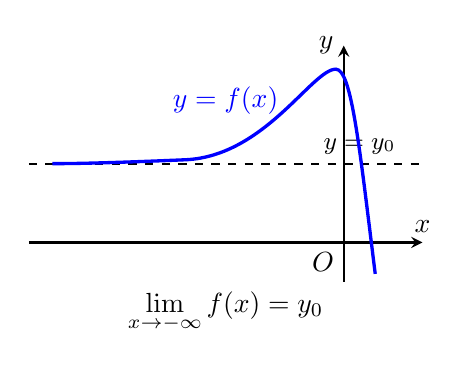
\begin{tikzpicture}[scale=1.0, >=stealth]
            % Axes
            \draw[->, thick] (-4.5,0) -- (0.5,0) node[above] {$x$};
            \draw[->, thick] (-0.5,-0.5) -- (-0.5,2.5) node[left] {$y$};
            \node[below left] at (-0.5,0) {$O$};
            
            % Dashed horizontal line y = y_0
            \draw[dashed, thick] (-4.5,1.0) -- (0.5,1.0);
            \node[above, font=\small] at (-0.3,1.0) {$y = y_0$};
            
            % Curve
            \draw[blue, very thick] (-4.2, 1.0) 
                .. controls (-3.8, 1.0) and (-3.2, 1.02) .. (-2.5, 1.05) 
                .. controls (-1.5, 1.1) and (-0.9, 2.2) .. (-0.6, 2.2) 
                .. controls (-0.4, 2.2) and (-0.3, 1.2) .. (-0.1, -0.4);
            \node[blue, above] at (-2.0, 1.5) {$y = f(x)$};
            
            % Limit label underneath
            \node[below=0.5cm] at (-2.0,0) {$\displaystyle\lim_{x \to -\infty} f(x) = y_0$};
        \end{tikzpicture}
    \end{minipage}
\end{center}
\vspace{0.8cm}
\subsection*{2. Đường tiệm cận đứng}
\begin{minipage}{0.55\textwidth}
    \begin{doublelinebox}
        Đường thẳng $x = x_0$ được gọi là đường tiệm cận đứng của đồ thị hàm số $y = f(x)$ nếu ít nhất một trong các điều kiện sau được thoả mãn:
        \[
        \lim_{x \to x_0^-} f(x) = +\infty; \quad \lim_{x \to x_0^-} f(x) = -\infty;
        \]
        \[
        \lim_{x \to x_0^+} f(x) = +\infty; \quad \lim_{x \to x_0^+} f(x) = -\infty.
        \]
    \end{doublelinebox}
\end{minipage}
\hfill
\begin{minipage}{0.4\textwidth}
    \centering
    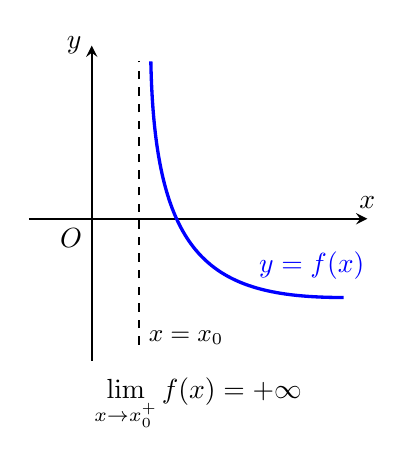
\begin{tikzpicture}[scale=1.0, >=stealth]
        % Axes
        \draw[->, thick] (-0.8,0) -- (3.5,0) node[above] {$x$};
        \draw[->, thick] (0,-1.8) -- (0,2.2) node[left] {$y$};
        \node[below left] at (0,0) {$O$};
        
        % Dashed vertical line x = x_0
        \draw[dashed, thick] (0.6,-1.6) -- (0.6,2.0);
        \node[below right, font=\small] at (0.6,-1.3) {$x = x_0$};
        
        % Curve
        \draw[blue, very thick] (0.75, 2.0) 
            .. controls (0.8, -0.5) and (1.5, -1.0) .. (3.2, -1.0);
        \node[blue, right] at (2.0,-0.6) {$y = f(x)$};
        
        % Limit label underneath
        \node[below=0.6cm] at (1.35,-1.3) {$\displaystyle\lim_{x \to x_0^+} f(x) = +\infty$};
    \end{tikzpicture}
\end{minipage}
\subsection*{3. Đường tiệm cận xiên}

\begin{minipage}{0.55\textwidth}
    \begin{doublelinebox}
        Đường thẳng $y = ax + b$ ($a \neq 0$) được gọi là đường tiệm cận xiên của đồ thị hàm số $y = f(x)$ nếu:
        \[
        \lim_{x \to +\infty} [f(x) - (ax + b)] = 0
        \]
        hoặc
        \[
        \lim_{x \to -\infty} [f(x) - (ax + b)] = 0.
        \]
    \end{doublelinebox}
\end{minipage}
\hfill
\begin{minipage}{0.4\textwidth}
    \centering
    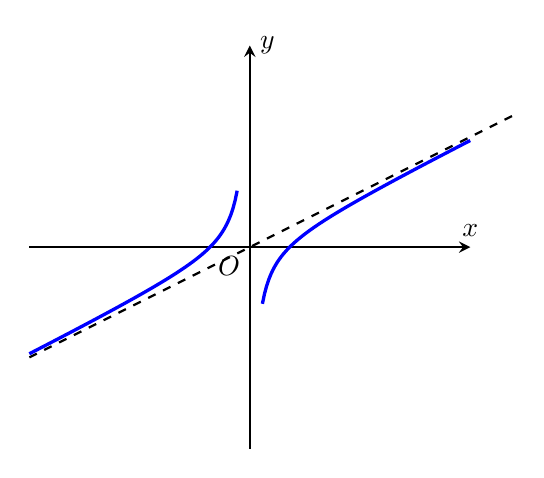
\begin{tikzpicture}[scale=0.8, >=stealth]
        % Hệ trục tọa độ
        \draw[->, thick] (-3.5,0) -- (3.5,0) node[above] {$x$};
        \draw[->, thick] (0,-3.2) -- (0,3.2) node[right] {$y$};
        \node[below left] at (0,0) {$O$};
        
        % Đường tiệm cận xiên nét đứt y = 0.5x
        \draw[dashed, thick] (-3.5,-1.75) -- (4.2,2.1);
        
        % Nhánh bên trái của đồ thị (x < 0)
        \draw[blue, very thick, domain=-3.5:-0.2, samples=100] 
            plot (\x, {0.5*\x - 0.2/\x});
            
        % Nhánh bên phải của đồ thị (x > 0)
        \draw[blue, very thick, domain=0.2:3.5, samples=100] 
            plot (\x, {0.5*\x - 0.2/\x});
    \end{tikzpicture}
\end{minipage}

\vspace{0.5cm}
\noindent Để xác định hệ số $a, b$ của đường tiệm cận xiên $y = ax + b$ của đồ thị hàm số $y = f(x)$, ta có thể áp dụng công thức sau:
\[
a = \lim_{x \to +\infty} \frac{f(x)}{x} \quad \text{và} \quad b = \lim_{x \to +\infty} [f(x) - ax]
\]
hoặc
\[
a = \lim_{x \to -\infty} \frac{f(x)}{x} \quad \text{và} \quad b = \lim_{x \to -\infty} [f(x) - ax].
\]

\end{document}